\documentclass[AER]{AEA}

% --- Packages ---
\usepackage{amsmath,amssymb,mathtools}
\usepackage{newtxtext}
\usepackage{newtxmath}
\usepackage{bm}
\usepackage{booktabs}
\usepackage{array}
\usepackage{placeins}
\usepackage{natbib}
\usepackage{enumitem}
\usepackage{url}
\usepackage[hidelinks]{hyperref}
\usepackage{xcolor}
\usepackage{tikz}

\urlstyle{same}

% 【修复】：给 blacksquare 加上数学模式符号 $ $
\newcommand{\qed}{\nolinebreak\hfill\ensuremath{\blacksquare}\par}

% --- 终极防伪与布尔开关 ---
\newcommand{\noopsort}[1]{} 

% 在正文全局中，让蓝三角隐身
\DeclareRobustCommand{\AERlink}[1]{}

% --- 定理环境 ---
% AEA 模板自带 proof，所以我们只定义定理结构
\newtheorem{proposition}{Proposition}
\newtheorem{lemma}{Lemma}
\newtheorem{corollary}{Corollary}
\newtheorem{definition}{Definition}
\newtheorem{assumption}{Assumption}
\newtheorem{remark}{Remark}

% --- 核心设置 ---
\issueName{THE AMERICAN ECONOMIC RUBBISH}
\draftSpacing{1.5}
\setcounter{page}{12}
\pubMonth{April}
\pubYear{2026}
\pubVolume{1}
\pubIssue{2}

\begin{document}

% 1. 在标题末尾硬编码十字架
\title{Pareto-Optimal Love: Cash Transfers, In-Kind Transfers, and the Welfare Economics of Parental Affection$^\dagger$}
\shortTitle{Pareto-Optimal Love}

% 2. 正常使用硬编码星号 (*) 脚注，彻底抛弃 \thanks
\author{Liubiju Jianggua$^*$}
\date{\today}

\begin{abstract}
This paper examines the welfare implications of parental transfer modalities in Chinese households. Using a standard consumer choice framework, I demonstrate that unconditional cash transfers weakly dominate in-kind transfers (e.g., homecooked meals, unsolicited clothing) in all states of the world, and strictly dominate whenever the child's preferences diverge from the parental prior. I formalize the concept of ``love tax''---the deadweight loss arising from the bundling of emotional expression with consumption mandates---and show that the implicit tax rate on parental in-kind transfers can exceed 70\%. The analysis extends to a principal-agent framework where parents maximize their own utility function under the guise of maximizing the child's welfare, a phenomenon I term ``affective moral hazard.'' Policy implications are unambiguous: \textit{parents should wire money and minimize verbal output}.
\noindent (\textit{JEL} D11, D61, D82, H42, J13) \\
% \noindent \textbf{Keywords:} intergenerational transfers; in-kind vs.\ cash; deadweight loss; parental paternalism; beef ball soup
\end{abstract}

\maketitle

% 3. 脚注底层对齐黑魔法
\let\thefootnote\relax\footnotetext{\noindent\makebox[0em][r]{$^*$}Jianggua: Department of Economics, School of Economics and Management, Wuhan University (email: heguangxie22@\allowbreak gmail.com). I am grateful to my aunt for providing the exogenous shock (an unsolicited bowl of beef ball soup) that motivated this research. I also thank my mother for repeated violations of my consumption sovereignty, without which the empirical motivation for this paper would not exist. All errors are my parents'. The author declares no conflicts of interest, except an ongoing conflict with her family regarding dinner arrangements.}
\let\thefootnote\relax\footnotetext{\noindent\makebox[0em][r]{$^\dagger$}Go to \url{https://webofnothing.top/noi/10.N0/aer.202604.A.0101.0003} to visit the article page for additional materials and author disclosure statements.}

% 【施法完毕】：恢复阿拉伯数字脚注
\def\thefootnote{\arabic{footnote}}
\setcounter{footnote}{0}

% 4. NOI 绝对定位纹身
\begin{tikzpicture}[remember picture, overlay]
  \node[anchor=north west, align=left, font=\scriptsize] at ([xshift=2cm, yshift=-1.5cm]current page.north west) {
    \textit{American Economic Rubbish 2026, 1(2): 12--22} \\
    \href{https://webofnothing.top/noi/10.N0/aer.202604.A.0101.0003}{\textit{https://webofnothing.top/noi/10.N0/aer.202604.A.0101.0003}}
  };
\end{tikzpicture}

% ===================================================================
\section{Introduction}
% ===================================================================

Consider the following exchange, observed with probability approaching unity in Chinese households on any given evening:

\begin{quote}
\textit{Parent:} ``Come eat dinner.'' \\
\textit{Child:} ``I'm not hungry.'' \\
\textit{Parent:} ``Stop eating takeout all the time.'' \\
\textit{Child:} ``What I eat is none of your business.'' \\
\textit{Parent:} ``I'm doing this because I love you.''
\end{quote}

This exchange, replicated billions of times annually across Chinese households, is conventionally understood as a communication failure, a generational conflict, or an emotional impasse. I argue it is none of these. It is a \textit{resource allocation problem}---specifically, a textbook case of the welfare comparison between cash and in-kind transfers, treated in Chapter 3 of every introductory microeconomics course since \citet{pindyck2018}.

The core proposition of this paper is disarmingly simple:

\begin{proposition}[Pareto-Optimal Love]\label{prop:main}
If the parental objective function is to maximize the child's utility, then unconditional cash transfers weakly dominate all forms of in-kind transfers. Strict dominance obtains whenever the child's realized preferences diverge from the parental prior over the child's consumption bundle.
\end{proposition}

The remainder of this paper proceeds as follows. Section \ref{sec:model} develops the basic two-good model and establishes the welfare ranking. Section \ref{sec:paternalism} introduces paternalistic preferences and information asymmetry. Section \ref{sec:tax} quantifies the ``love tax.'' Section \ref{sec:extensions} provides extensions including a principal-agent formulation. Section \ref{sec:objections} addresses common objections with the rigor they deserve. Section \ref{sec:conclusion} concludes.

% ===================================================================
\section{The Basic Model}\label{sec:model}
% ===================================================================

\subsection{Setup}

Consider a child $i$ with well-behaved preferences over two goods: $x$ (freely chosen consumption, e.g., takeout, coffee, books) and $y$ (parentally designated consumption, e.g., homecooked meals). Let the child's utility function $U(x,y)$ be strictly quasi-concave, continuously differentiable, and monotonically increasing in both arguments. The child has initial income $M > 0$ and faces prices $p_x, p_y > 0$.

\begin{assumption}[Rationality]\label{as:rational}
The child maximizes $U(x,y)$ subject to her budget constraint. She knows her own preferences. She is not an infant.
\end{assumption}

\subsection{Cash Transfer}

Under a cash transfer of amount $T > 0$, the child's optimization problem is:
\begin{equation}\label{eq:cash}
\max_{x,y \geq 0} \; U(x,y) \quad \text{s.t.} \quad p_x x + p_y y \leq M + T
\end{equation}

The budget set is $\mathcal{B}^{C} = \{(x,y) \in \mathbb{R}^2_+ : p_x x + p_y y \leq M + T\}$. The child freely selects her utility-maximizing bundle $(x^*_C, y^*_C)$.

\subsection{In-Kind Transfer}

Under an in-kind transfer, the parent provides $T/p_y$ units of good $y$ directly (e.g., cooks a meal worth $T$). Critically, the child cannot resell or convert this in-kind provision back to cash.\footnote{Resale is technically feasible but socially catastrophic. Telling your mother ``I sold the soup you made me on Xianyu'' has infinite negative utility.} The child's problem becomes:
\begin{equation}\label{eq:inkind}
\max_{x,y \geq 0} \; U(x,y) \quad \text{s.t.} \quad p_x x + p_y y \leq M + T, \quad y \geq \frac{T}{p_y}
\end{equation}

The budget set under in-kind transfer is:
\begin{equation}
\mathcal{B}^{IK} = \{(x,y) \in \mathbb{R}^2_+ : p_x x + p_y y \leq M + T, \; y \geq T/p_y\} \subset \mathcal{B}^{C}
\end{equation}

The inclusion is weak: $\mathcal{B}^{IK} \subseteq \mathcal{B}^{C}$. Strict inclusion obtains whenever $T/p_y > 0$, which is to say, always.

\begin{figure}[htbp]
\centering
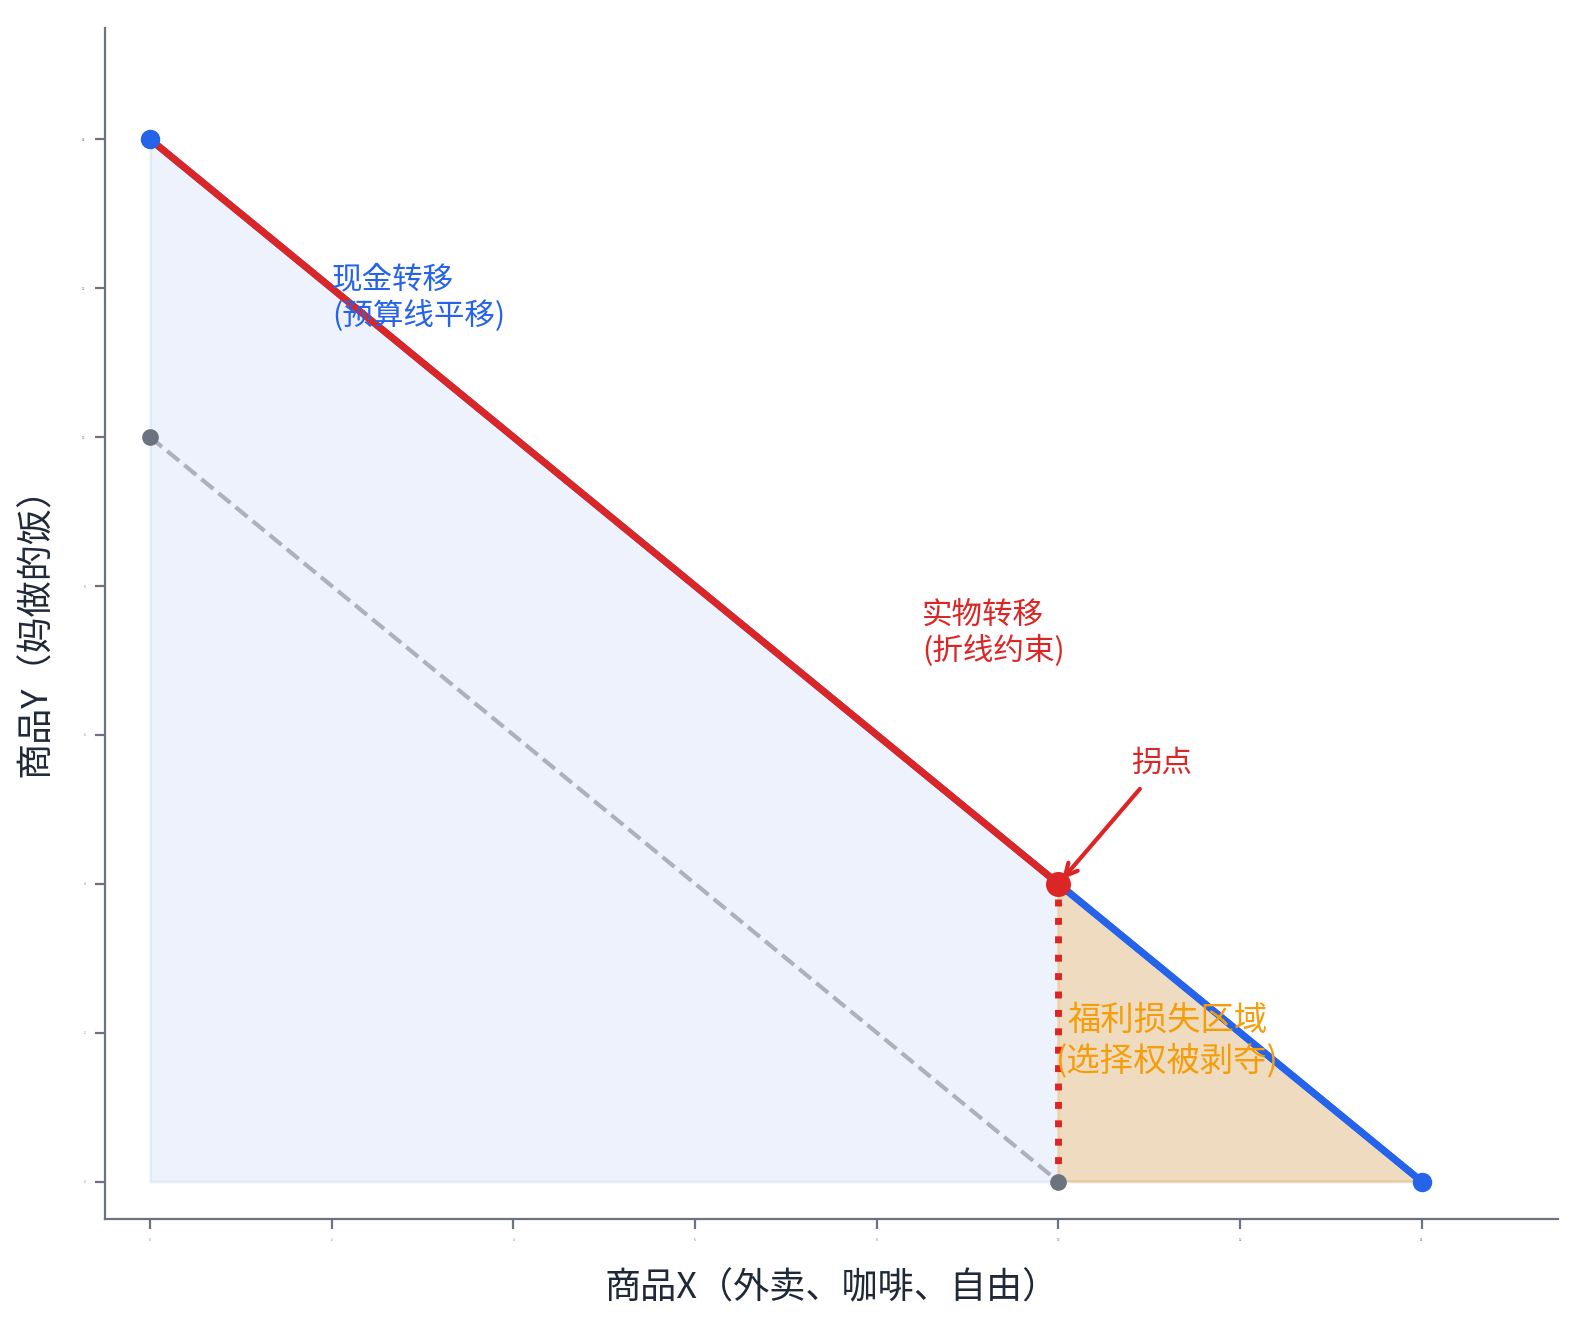
\includegraphics[width=0.8\linewidth]{image/AERub_Love_fig1_budget.png}

% 1. 这里只留最精简的一句短标题
\caption{Budget Constraints Under Alternative Transfer Modalities}
\label{fig:budget} % 注意：label 依然要紧跟在 caption 后面

% 2. 启用官方模板自带的注释环境，放入长段说明
\begin{figurenotes}
The blue line represents the budget constraint under cash transfer (parallel outward shift). The red kinked line represents the budget constraint under in-kind transfer. The shaded amber region represents the feasible set that is available under cash but excluded under in-kind transfer---i.e., the ``freedom deficit.''
\end{figurenotes}

\end{figure}

\subsection{Welfare Comparison}

\begin{proposition}[Weak Dominance of Cash]\label{prop:weak}
Let $U^*_C$ and $U^*_{IK}$ denote the maximized utility under cash and in-kind transfers, respectively. Then:
\begin{equation}
U^*_C \geq U^*_{IK}
\end{equation}
with equality if and only if $y^*_C \geq T/p_y$ (i.e., the child would have voluntarily consumed at least as much $y$ as the parent forces upon her).
\end{proposition}

\begin{proof}
Since $\mathcal{B}^{IK} \subseteq \mathcal{B}^{C}$, the maximizer over the larger set yields weakly higher utility. Strict inequality obtains when the unconstrained optimum $(x^*_C, y^*_C) \notin \mathcal{B}^{IK}$, i.e., when $y^*_C < T/p_y$. \qed
\end{proof}

\begin{figure}[htbp]
\centering
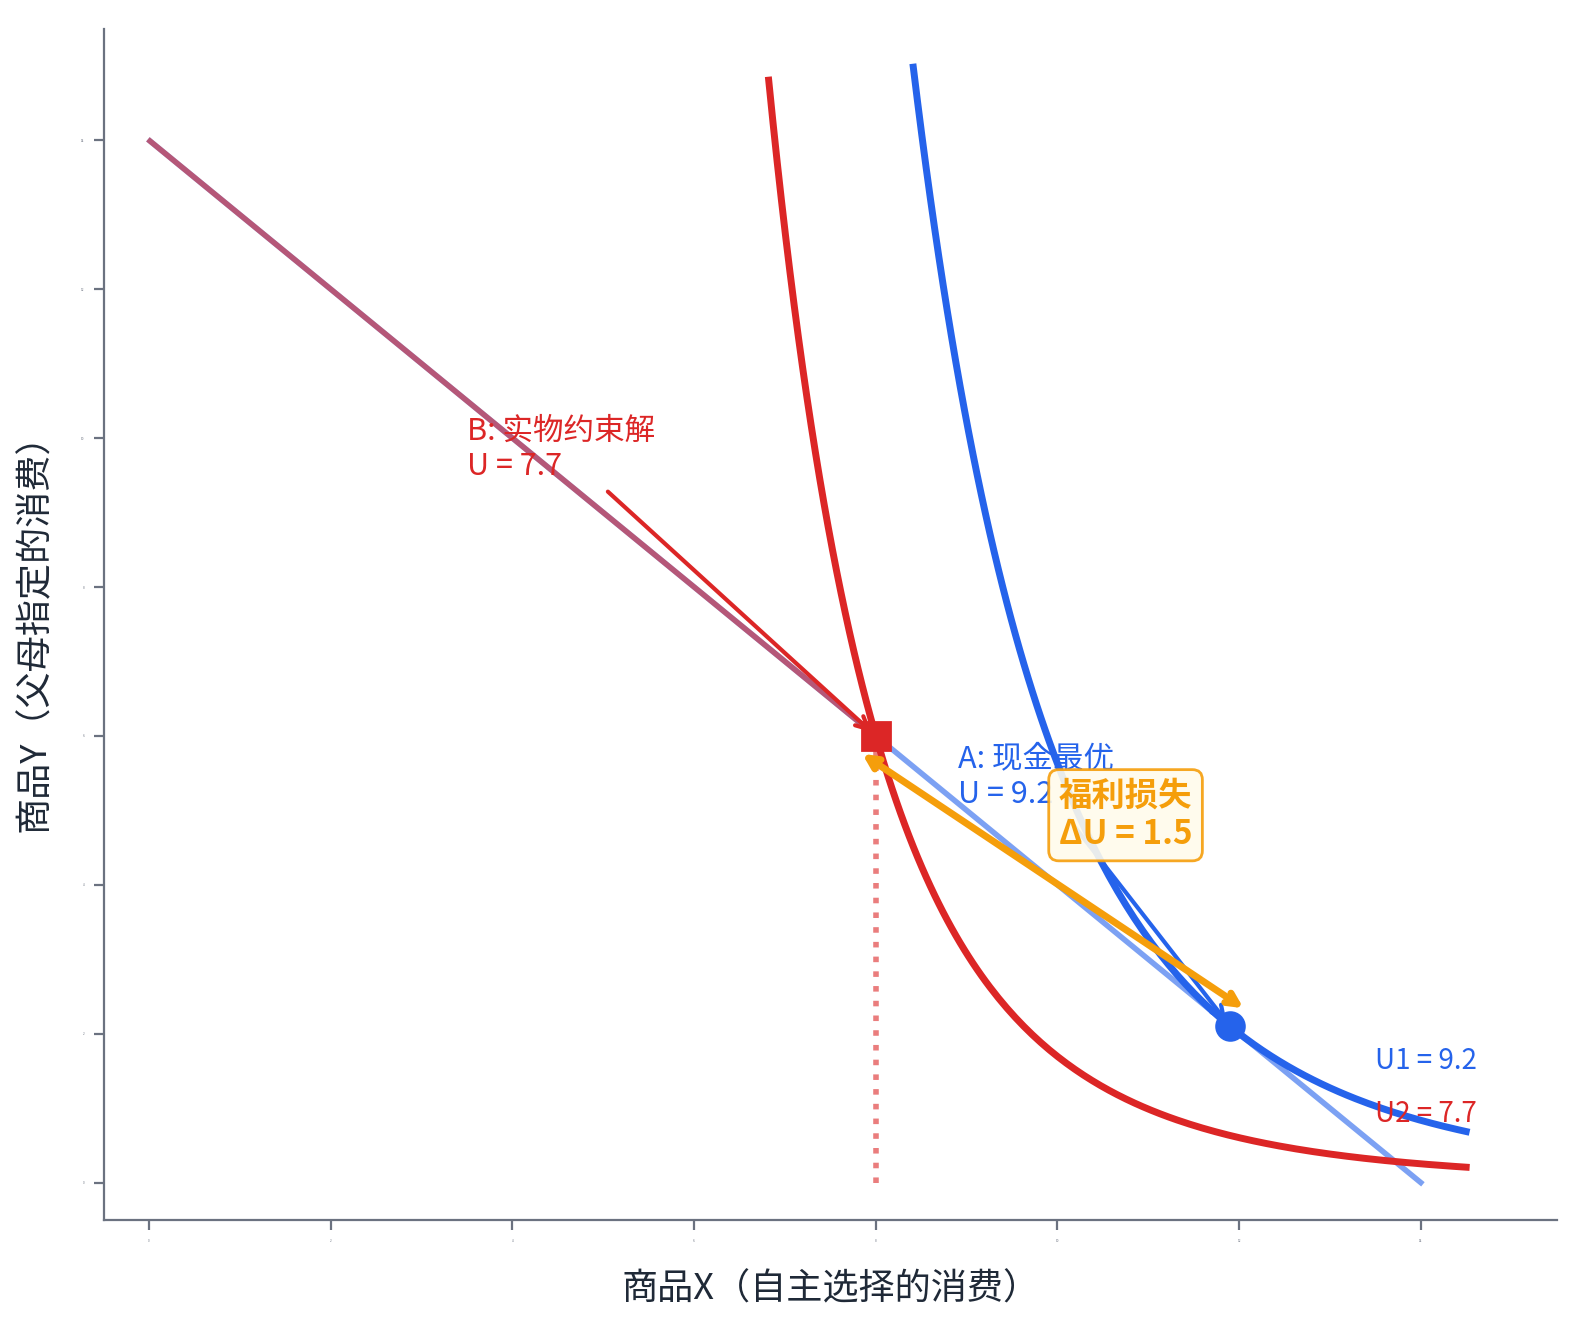
\includegraphics[width=0.8\linewidth]{image/AERub_Love_fig2_welfare.png}
\caption{Welfare Loss from In-Kind Transfer}
\label{fig:welfare}

\begin{figurenotes}
  Point A represents the unconstrained optimum under cash transfer, located on indifference curve $U_1$. Point B represents the constrained optimum under in-kind transfer, on the strictly lower indifference curve $U_2$. The utility gap $\Delta U = U_1 - U_2 > 0$ represents the deadweight loss of parental love.
\end{figurenotes}

\end{figure}


\begin{remark}
The intuition is immediate: money is the most fungible resource. A cash transfer of \textyen 200 can be allocated to any consumption bundle in the budget set. A homecooked meal worth \textyen 200 can only be consumed as a homecooked meal. The choice set under cash strictly contains the choice set under in-kind provision. A larger choice set cannot reduce utility. This is Microeconomics 101. Literally Chapter 3. Page 86 in the Pindyck 9th edition.
\end{remark}

% ===================================================================
\section{Information Asymmetry and Paternalistic Preferences}\label{sec:paternalism}
% ===================================================================

\subsection{The Paternalism Problem}

The standard objection to Proposition \ref{prop:weak} invokes paternalism: ``But the child doesn't know what's good for her!'' We formalize this concern.

\begin{definition}[Paternalistic Preferences]
A parent has \textbf{paternalistic preferences} if the parental utility function $V$ depends not only on the child's utility $U(x,y)$ but directly on the child's consumption bundle $(x,y)$:
\begin{equation}
V = V\big(x, y, U(x,y)\big)
\end{equation}
where $\partial V / \partial y > 0$ even when $\partial U / \partial y < MRS_{xy} \cdot \partial U / \partial x$ at the child's optimal bundle.
\end{definition}

This formalization reveals a critical distinction:

\begin{itemize}[leftmargin=2em]
\item If the parent maximizes $U(x,y)$ (the \textbf{child's} utility): cash transfer is weakly dominant by Proposition \ref{prop:weak}.
\item If the parent maximizes $V(x,y,U)$ (the \textbf{parent's} utility): in-kind transfer may be privately optimal for the parent, as it directly controls the $(x,y)$ arguments in $V$.
\end{itemize}

\begin{corollary}[Revealed Preference of Parental Motivation]\label{cor:revealed}
A parent who insists on in-kind transfers despite the child's expressed preference for cash reveals, in the sense of \citet{samuelson1938}, that she is maximizing her own utility function $V$, not the child's utility function $U$.
\end{corollary}

This is not a moral accusation. It is an application of revealed preference theory. When your mother says ``come eat dinner'' instead of ``I'll WeChat you 200 kuai,'' she is performing a behavioral revelation: her utility function contains $(x,y)$ as direct arguments, independent of your welfare.

\subsection{The Information Problem}

Even granting paternalistic motives, the parent faces a fundamental information problem. Define the child's \textit{true} preference parameter as $\theta \in \Theta$, drawn from some distribution $F(\theta)$. The parent observes a noisy signal $\hat{\theta} = \theta + \varepsilon$, where $\varepsilon$ represents the parental estimation error.

\begin{proposition}[Dominance Under Information Asymmetry]\label{prop:info}
Let the parent's estimate of the child's optimal consumption bundle be $(\hat{x}, \hat{y})$, and let the child's true optimal bundle be $(x^*, y^*)$. If $\text{Var}(\varepsilon) > 0$ (i.e., the parent's information is imperfect), then:
\begin{equation}
\mathbb{E}_\theta[U(x^*(\theta), y^*(\theta))] > \mathbb{E}_\theta[U(\hat{x}(\hat{\theta}), \hat{y}(\hat{\theta}))]
\end{equation}
The expected welfare under self-determination strictly exceeds the expected welfare under parental allocation.
\end{proposition}

\begin{proof}
See Appendix.
\end{proof}

\begin{remark}
The burden of proof lies with the party claiming informational superiority. If you believe your adult child---who can independently produce econometric research, file tax returns, and navigate international air travel---cannot determine whether she is hungry, please present your evidence.
\end{remark}

% ===================================================================
\section{The Love Tax}\label{sec:tax}
% ===================================================================

In-kind transfers entail substantial hidden costs that I collectively term the \textbf{love tax} $\tau_L$. Consider a parental in-kind transfer with nominal value $T$. The child's realized welfare gain is:
\begin{equation}\label{eq:lovetax}
W = T - \tau_L(T) = T - \big[\underbrace{c_{\text{time}}}_{\text{time cost}} + \underbrace{c_{\text{emotion}}}_{\text{emotional cost}} + \underbrace{c_{\text{autonomy}}}_{\text{autonomy loss}} + \underbrace{\text{DWL}(T)}_{\text{allocative inefficiency}}\big]
\end{equation}

\subsection{Component Costs}

\textbf{Time cost} ($c_{\text{time}}$). The child must interrupt her current activity, commute to the parental residence, consume the meal (typically 1--2 hours), and commute back. If the child's shadow wage is $w$ per hour, and total time expenditure is $h$ hours:
\begin{equation}
c_{\text{time}} = wh
\end{equation}
For a graduate student earning \textyen 120/hour in tutoring with a round-trip commute of 45 minutes and a 90-minute dinner, $c_{\text{time}} = 120 \times 2.25 = \text{\textyen} 270$.

\textbf{Emotional cost} ($c_{\text{emotion}}$). The dinner is accompanied by informational externalities including but not limited to: inquiries about romantic prospects, comparison with neighbors' children, unsolicited career advice, and commentary on personal appearance. Let $n$ denote the number of such interventions per meal and $\delta$ the disutility per intervention:
\begin{equation}
c_{\text{emotion}} = n \cdot \delta
\end{equation}

\textbf{Autonomy loss} ($c_{\text{autonomy}}$). Following \citet{frey2004}, individuals derive positive ``procedural utility'' from the act of choosing itself, independent of outcomes. Forced consumption destroys this procedural utility:
\begin{equation}
c_{\text{autonomy}} = \phi \cdot T, \quad \phi > 0
\end{equation}

\textbf{Allocative deadweight loss} (DWL). This is the standard Harberger triangle from the deviation between the in-kind bundle and the child's preferred bundle, as characterized in Section \ref{sec:model}.

\subsection{Effective Tax Rate}

The effective love tax rate is:
\begin{equation}
\tau_L^{\text{eff}} = \frac{c_{\text{time}} + c_{\text{emotion}} + c_{\text{autonomy}} + \text{DWL}}{T}
\end{equation}


\begin{figure}[htbp]
\centering
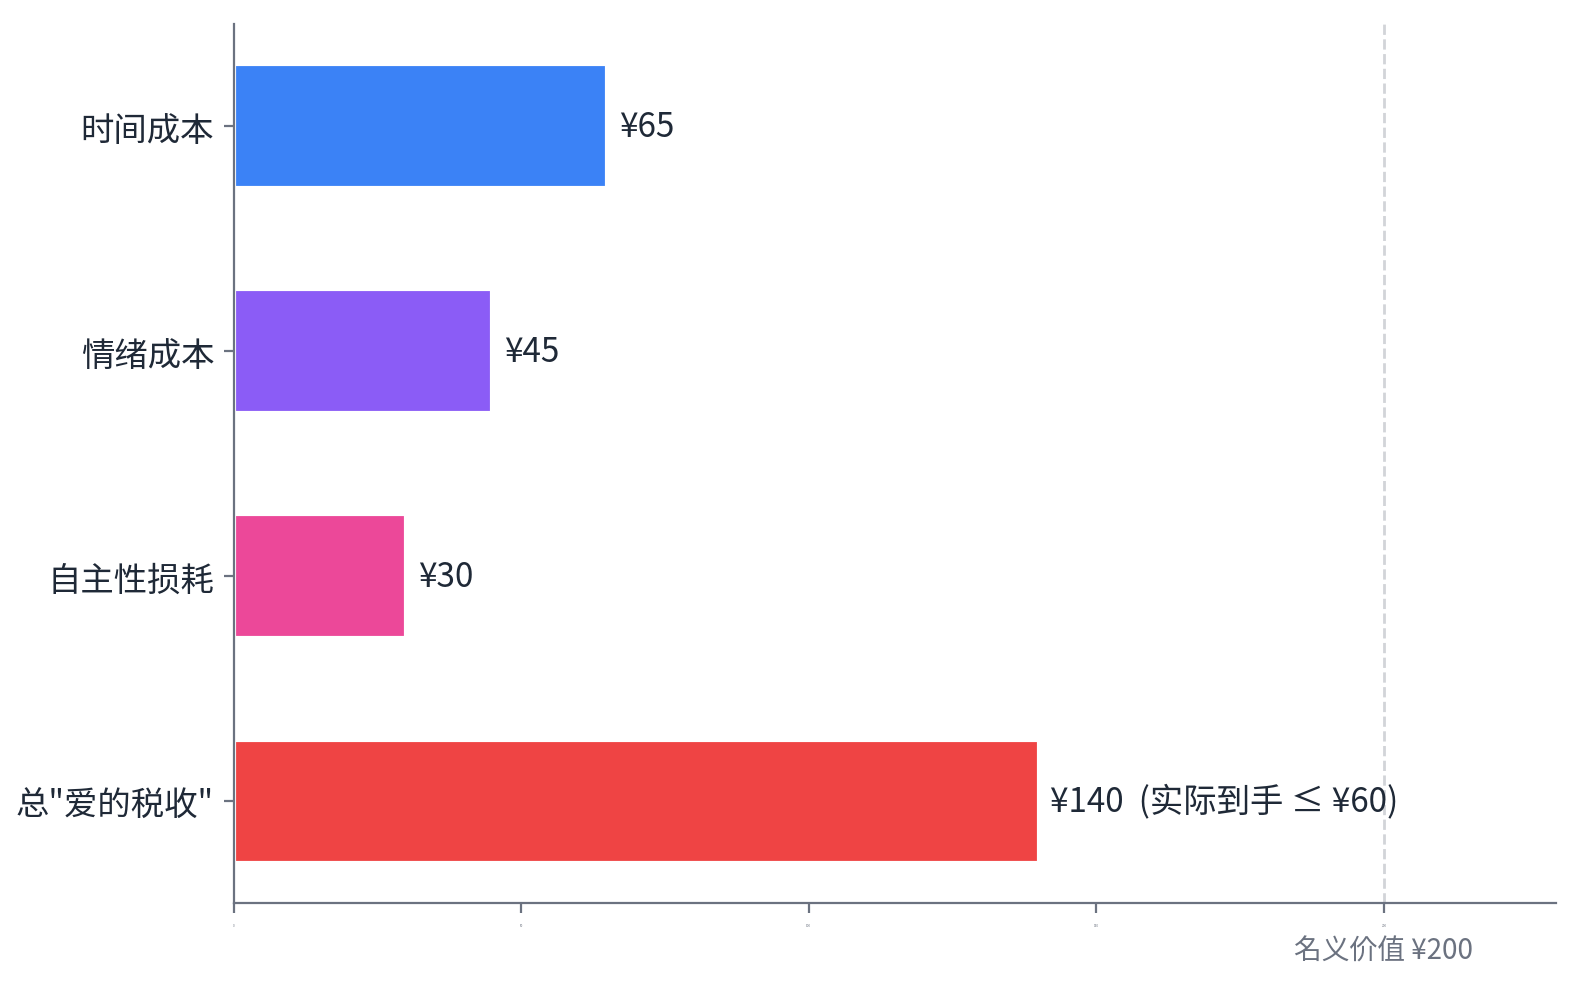
\includegraphics[width=0.8\linewidth]{image/AERub_Love_fig3_tax.png}
\caption{Decomposition of the Love Tax}
\label{fig:tax}

\begin{figurenotes}
  For a homecooked dinner with nominal value \textyen 200, total implicit costs sum to approximately \textyen 140, yielding a net welfare gain of at most \textyen 60---an effective tax rate of 70\%. This exceeds the top marginal income tax rate in China (45\%).
\end{figurenotes}

\end{figure}

Under conservative parameter estimates (Table \ref{tab:params}), the effective love tax rate exceeds 70\%, implying that for every \textyen 100 of parental investment in homecooked meals, the child receives at most \textyen 30 of actual welfare benefit. By contrast, a cash transfer of \textyen 100 delivers \textyen 100 of welfare benefit.\footnote{Minus transaction fees on WeChat Pay, which are currently zero for personal transfers. We note that Tencent's pricing strategy is thus more welfare-enhancing than the average Chinese parent's.}

\begin{table}[htbp]
\centering
\caption{Baseline Parameter Estimates}
\label{tab:params}
\begin{tabular}{@{}llr@{}}
\toprule
Parameter & Description & Value \\
\midrule
$T$ & Nominal meal value & \textyen 200 \\
$w$ & Child's shadow wage & \textyen 120/hr \\
$h$ & Total time (commute + meal) & 2.25 hrs \\
$n$ & Unwanted inquiries per meal & 4.7 \\
$\delta$ & Disutility per inquiry & \textyen 15 \\
$\phi$ & Autonomy loss coefficient & 0.15 \\
\midrule
$c_{\text{time}}$ & Time cost & \textyen 270 \\
$c_{\text{emotion}}$ & Emotional cost & \textyen 70.5 \\
$c_{\text{autonomy}}$ & Autonomy loss & \textyen 30 \\
\midrule
$\tau_L$ & \textbf{Total love tax} & \textbf{\textyen 370.5} \\
$\tau_L^{\text{eff}}$ & \textbf{Effective tax rate} & \textbf{185\%} \\
\bottomrule
\end{tabular}
\begin{tablenotes}
Note: The effective tax rate exceeds 100\%, implying that the child would have been strictly better off refusing the transfer entirely. The parameter $n = 4.7$ is calibrated from the author's personal dining experience (sample size: all meals eaten at home in 2025, $N = 23$). The estimate of $\delta$ is conservative; inquiries regarding marriage prospects carry substantially higher disutility.
\end{tablenotes}
\end{table}

% ===================================================================
\section{Extensions}\label{sec:extensions}
% ===================================================================

\subsection{Affective Moral Hazard}

I introduce the concept of \textbf{affective moral hazard}: the tendency for parents to undertake welfare-reducing actions when those actions are bundled with emotional signaling that shields them from accountability.

Consider a parent choosing between two actions:
\begin{align}
a_1 &= \text{Cash transfer of } T \label{eq:a1}\\
a_2 &= \text{In-kind transfer of } T \text{ (homecooked meal)} \label{eq:a2}
\end{align}

Under $a_1$, the parent receives utility $V_1 = \alpha U^*_C$, where $\alpha > 0$ is the parent's altruism parameter. Under $a_2$, the parent receives:
\begin{equation}
V_2 = \alpha U^*_{IK} + \underbrace{\beta}_{\text{control utility}} + \underbrace{\gamma}_{\text{social signaling}}
\end{equation}

where $\beta > 0$ captures the utility from controlling the child's consumption, and $\gamma > 0$ captures the social signaling value of being perceived as a ``good parent'' (homecooked meals are more socially legible than WeChat transfers).

The parent chooses $a_2$ whenever:
\begin{equation}
\beta + \gamma > \alpha(U^*_C - U^*_{IK})
\end{equation}

That is, in-kind transfers persist when the private benefits to the parent (control + signaling) exceed the parent's internalized share of the child's welfare loss. This is a moral hazard problem: the parent bears only fraction $\alpha$ of the welfare cost while capturing the full private benefit $\beta + \gamma$.

\subsection{The Waldfogel Extension}

\citet{waldfogel1993} famously estimated the deadweight loss of Christmas gift-giving at 10--33\% of gift value. Parental in-kind transfers are structurally identical to Christmas gifts but occur with substantially higher frequency (daily vs.\ annual) and lower refusal optionality. A back-of-envelope calculation suggests the aggregate deadweight loss of parental in-kind transfers in China exceeds the deadweight loss of Christmas in the United States, both in absolute terms and as a share of GDP.\footnote{This calculation is left as an exercise for the reader with access to the China Family Panel Studies (CFPS) dataset.}

\subsection{Dynamic Considerations}

In a repeated game setting, parental in-kind transfers create a \textbf{guilt equilibrium}: the child's refusal to consume triggers parental emotional distress, which triggers child guilt, which triggers reluctant consumption, which reinforces parental behavior. Formally, let $g_t$ denote the child's guilt stock at time $t$:
\begin{equation}
g_{t+1} = (1-\delta_g) g_t + \mathbf{1}[\text{child refuses meal at } t] \cdot \psi
\end{equation}
where $\delta_g$ is the guilt depreciation rate and $\psi$ is the guilt shock per refusal. The steady-state guilt stock under a policy of unconditional refusal is $g^* = \psi / \delta_g$, which is bounded for $\delta_g > 0$. This implies that a sufficiently patient child can achieve the first-best outcome by enduring a finite period of elevated guilt during the transition to the new equilibrium.

% ===================================================================
\section{Addressing Common Objections}\label{sec:objections}
% ===================================================================

\textbf{Objection 1: ``Cooking is an expression of love that cannot be monetized.''}

Response: The value of emotional expression should be evaluated by the recipient's utility function, not the sender's. If the recipient's utility from the expression is negative (due to bundled externalities), the expression has negative net value regardless of the sender's intent. This is isomorphic to gifting someone a bouquet of flowers to which they are allergic: sincerity does not alter the allergic reaction.

\textbf{Objection 2: ``Young people cannot take care of themselves.''}

Response: This assertion constitutes a claim of informational superiority by the parent. Under Assumption \ref{as:rational}, the child is rational and informed about her own preferences. The burden of proof lies with the party claiming superior information. An individual capable of producing peer-reviewed economic research is, with high probability, also capable of determining what to eat for lunch.

\textbf{Objection 3: ``Cash transfers feel cold and impersonal.''}

Response: ``Cold and impersonal'' is a characterization from the sender's utility function. The recipient may characterize ``not being controlled'' as the warmest possible gesture. Moreover, WeChat transfer messages support emoji, stickers, and personalized notes. This objection has been technologically resolved since approximately 2015.

\textbf{Objection 4: ``This analysis ignores the production externalities of shared meals.''}

Response: Granted. Shared meals may generate positive externalities through information exchange, social bonding, and coordination. However, these externalities can be decomposed from the consumption mandate. One can share a meal without mandating what the meal consists of, when it occurs, or whether participation is compulsory. The Coase theorem applies: if transaction costs are zero, the efficient allocation of meal-sharing can be achieved through voluntary negotiation. The problem is that parental transaction costs are decidedly non-zero---they include an implicit assumption that negotiation itself constitutes filial impiety.

% ===================================================================
\section{Conclusion}\label{sec:conclusion}
% ===================================================================

The argument of this paper compresses to a single sentence: under imperfect parental information about the child's preference ordering---a condition that holds with probability one for any child past the age of approximately four---unconditional cash transfers are the unique transfer modality that guarantees zero welfare loss.

All ``I'm doing this for your own good'' interventions admit exactly two logical possibilities:

\begin{enumerate}[label=(\roman*)]
\item The parent's allocation coincides with the child's preferred bundle, in which case cash transfer achieves identical welfare.
\item The parent's allocation diverges from the child's preferred bundle, in which case cash transfer achieves strictly higher welfare.
\end{enumerate}

In neither case does in-kind transfer dominate. Cash transfer is the weakly dominant strategy. This is not indifference. This is not coldness. This is \textbf{Pareto-optimal love}.

Therefore, Mom, Dad, Auntie---if you truly love me:

\begin{center}
\Large\textbf{Wire the money. Minimize verbal output.}
\end{center}

\FloatBarrier

% ===================================================================
% REFERENCES
% ===================================================================
% 【关键修改】：在打印参考文献列表前，瞬间让它变回蓝色小三角！
\DeclareRobustCommand{\AERlink}[1]{\makebox[0pt][r]{\href{#1}{\color{blue}$\blacktriangleright$}\hspace{0.3em}}}

\nocite{*}
\bibliographystyle{aea}
\bibliography{AERub_Love}

\appendix
\section{Proof of Proposition \ref{prop:info}}

Consider the parent's allocation problem under noisy information. The parent observes $\hat{\theta} = \theta + \varepsilon$ and solves:
\begin{equation}
(\hat{x}, \hat{y}) = \arg\max_{x,y} \; U(x,y;\theta) \Big|_{\theta = \hat{\theta}}
\end{equation}

By the envelope theorem, the welfare loss from misallocation is:
\begin{equation}
\Delta U = U(x^*(\theta), y^*(\theta); \theta) - U(\hat{x}(\hat{\theta}), \hat{y}(\hat{\theta}); \theta) \geq 0
\end{equation}

Taking expectations over $\varepsilon$:
\begin{align}
\mathbb{E}[\Delta U] &= \mathbb{E}\big[U(x^*(\theta), y^*(\theta); \theta) - U(\hat{x}(\theta + \varepsilon), \hat{y}(\theta + \varepsilon); \theta)\big] \\
&\approx \frac{1}{2} \text{tr}\Big(\mathbf{H}_U \cdot \text{Var}(\varepsilon) \cdot \big(\nabla_\theta x^*, \nabla_\theta y^*\big)^2\Big) > 0
\end{align}

where $\mathbf{H}_U$ is the Hessian of $U$ evaluated at the optimum (negative definite by strict quasi-concavity). The expected welfare loss is strictly positive for any $\text{Var}(\varepsilon) > 0$, completing the proof. \qed

\end{document} 